\documentclass[12 pt, a4paper]{article}
\usepackage[utf8]{inputenc}
\usepackage[letterpaper,top=2cm,bottom=2cm,left=3cm,right=3cm,marginparwidth=1.75cm]{geometry}
\usepackage[english, russian]{babel}
 \usepackage{graphicx}
 \usepackage{verbatim
 

\begin{document}
\begin{center}
\hfill \break
\large{МИНИСТЕРСТВО НАУКИ И ВЫСШЕГО ОБРАЗОВАНИЯ РОССИЙСКОЙ ФЕДЕРАЦИИ}\\
\footnotesize{Федеральное государственное автономное образовательное учреждение высшего образования}\\ 
\footnotesize{«Дальневосточный федеральный университет»}\\
\small{\textbf{(ДВФУ)}}\\
\hfill \break
\normalsize{ИНСТИТУТ МАТЕМАТИКИ И КОМПЬЮТЕРНЫХ ТЕХНОЛОГИЙ}\\
 \hfill \break
\normalsize{Департамент математического и компьютерного моделирования}\\
\hfill\break
\hfill \break
\hfill \break
\hfill \break
\large{Алгоритм Форчуна}\\
\hfill \break
\hfill \break
\hfill \break
\normalsize{Доклад\\
\hfill \break
Направление подготовки 09.03.03 Прикладная информатика\\
\hfill \break
Профиль «Приладная информатика в компьютерном дизайне»}\\
\hfill \break
\hfill \break
\end{center}
 
\normalsize{} \hfill \break
\hfill \break
 
\normalsize{ 
\begin{tabular}{cccc}
Обучающийся & \underline{\hspace{3cm}} & &А.В. Быкова \\\\
Руководитель & \underline{\hspace{3cm}}& доцент ИМКТ &А.С. Кленин \\\\
\end{tabular}
}\\
\hfill \break
\hfill \break
\begin{center} Владивосток 2022 \end{center}
\thispagestyle{empty} 
 
\newpage
     
    \tableofcontents 
\newpage

\section{Введение}
\subsection{Суть и назначение}
Алгоритм Форчуна – это алгоритм заметающей прямой для генерации диаграммы
Вороного из набора точек на плоскости за время O(n log n) с использованием памя-
ти O(n). Алгоритм берет множесто 2D-точек, которые вводятся заранее и строит по
ним диаграмму Вороного. Для каждой входной точки, которая называется «сай-
том», нам нужно найти множество точек, которые ближе к этому месту, чем ко
всем остальным. Такие множества точек образуют ячейки, множество которых и
называется диаграммой Вороного.
\subsection{Авторство}
Данный алгоритм был опубликован Стивеном Форчуном в 1986 году в Нью Джерси во время Второго ежегодного симпозиума по Компьютерной Геометрии. Статья носит название «A Sweepline Algorithm for Voronoi Diagrams» . Название алгоритма происходит от имени его создателя.
\subsection{История развития}
Алгоритм увидел свет в 1986 году, в статье математика Стивена Форчуна под названием «Алгоритм развертки линий для диаграмм Вороного». Ни один из просмотренных источников не содержит более подробной информации об этом событии, о его предшественниках или об авторе. Так же, отсюда можно сделать вывод, что до Стивена Форчуна никто не интересовался данной темой настолько, чтобы создать полноценный работающий алгоритм, собственно, как и после.
\subsection{Состояние, реализация}
На момент своего появления, алгоритм Форчуна был первым в своем роде, который строил диаграмму Вороного с использованием заметающей прямой. Поскольку информация об этом алгоритме ограничена, можно сделать вывод, что он не сыскал популярности в свое время. Возможно это произошло из-за сложности вычислений, а может и совсем по другим причинам.
\subsection{Перспектива Использования}
Алгоритм используется для построения диаграммы Вороного, которая в свою очередь имеет широкий спектр применения. 
Диаграммы Вороного постоянно использовались антропологами для описания регионов влияния различных культур; кристаллографами для объяснения структуры определенных кристаллов и металлов; экологами для изучения конкуренции между растениями; и экономистами для моделирования рынков в экономике США.Также, она используется в архитектуре, дизайне, поскольку образует красивые причудливые формы. 
\newpage
\section{Метод}
\subsection{Формальное описание метода}
Существует некоторое количество точек на плоскости - сайтов. Есть заметающая прямая, которая двигается (например) «сверху вниз», то есть от сайта с наибольшей ординатой к сайту с меньшей (от события к событию, если быть точным). Сразу стоит отметить, что влияние на построение диаграммы оказывают только те сайты, которые находятся выше или на заметающей прямой.
Когда ЗП попадает на очередной сайт (происходит событие точки (point event)), создаётся новая парабола (arch), фокусом которой является данный сайт, а директрисой — заметающая прямая. Эта парабола делит плоскость на две части — «внутренняя» область параболы соответствует точкам, которые сейчас ближе к сайту, а «внешняя» область — точкам, которые ближе к sweep line, ну а точки, лежащие на параболе — равноудалены от сайта и ЗП. Парабола будет меняться в зависимости от положения ЗП к сайту — чем дальше ЗП уходит от сайта вниз, тем больше расширяется парабола, однако в самом начале она вообще является отрезком («направленным» вверх). Далее парабола расширяется, у неё появляются две контрольные точки (break points) — точки её пересечения с остальными параболами («береговой линией»). В «береговой линии» мы храним дуги парабол от одной точки пересечения их друг с другом до другой, так и получается beach line. По сути, в этом алгоритме мы моделируем движение этой «береговой линии». потому как эти самые break point`ы движутся по рёбрам ячеек Вороного (ведь получается, что контрольные точки равноудалены от обоих сайтов, которым соответствуют эти параболы, да ещё и от ЗП).
И как раз-таки в тот момент, когда две контрольные точки — по одной из разных парабол — «встречаются», то есть как бы превращаются в одну, эта точка и становится вершиной ячейки Вороного (происходит событие круга (circle event)), причём в это время та дуга, которая находилась между этими двумя точками — «схлопывается» и удаляется из «береговой линии». Далее мы просто соединяем эту точку с предыдущей соответствующей ей и получаем ребро ячейки Вороного.

\newpage
\subsection{Математическое описание метода}
\subsection{Псевдокод}
Оригинальный всевдокод Стивена Форчуна:\\
\begin{align}
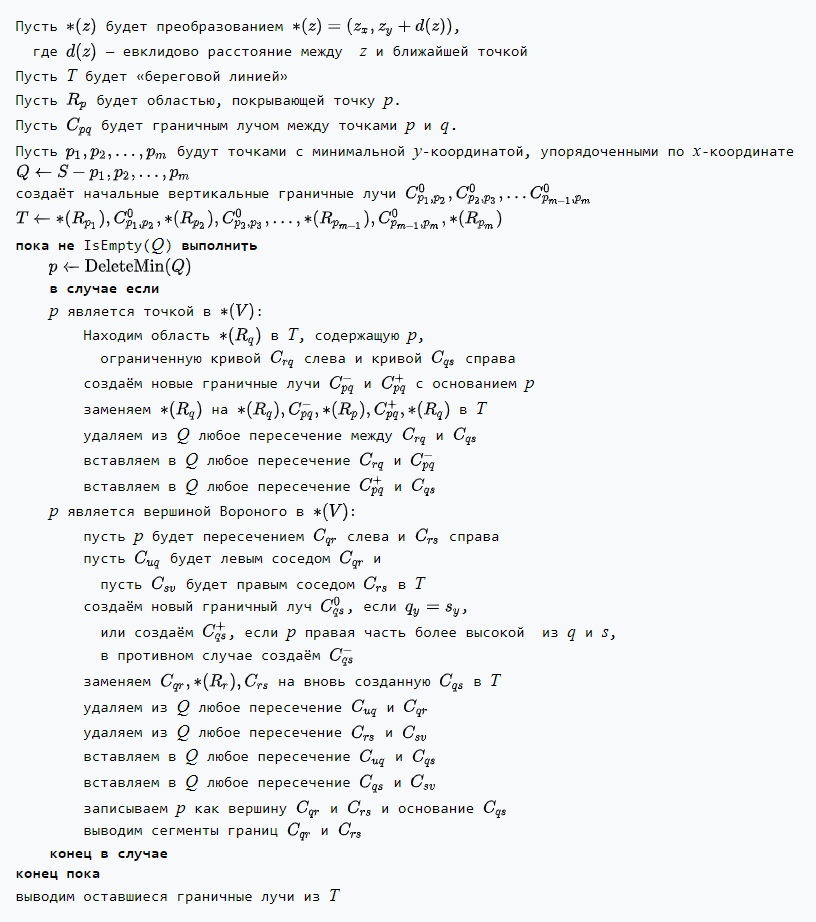
\includegraphics[scale = 0.55]{Псевдокод}
\end{center}
\newpage

\subsection{Пример}
Имеется поле с размерами: ширина – 1000, высота – 800. 
На ввод подаются 5 точек с координатами (208,235), (545,108), (342,601), (724,369), (455,352) соответственно. Программа считывает входные данные, располагает точки в местах, соответсвующих их координатам, проходит по ним сверху вниз заметающей прямой и строит диаграмму Вороного. На выход поступает визуальное отображение диаграммы Вороного, подобного вида:\\
\begin{center}
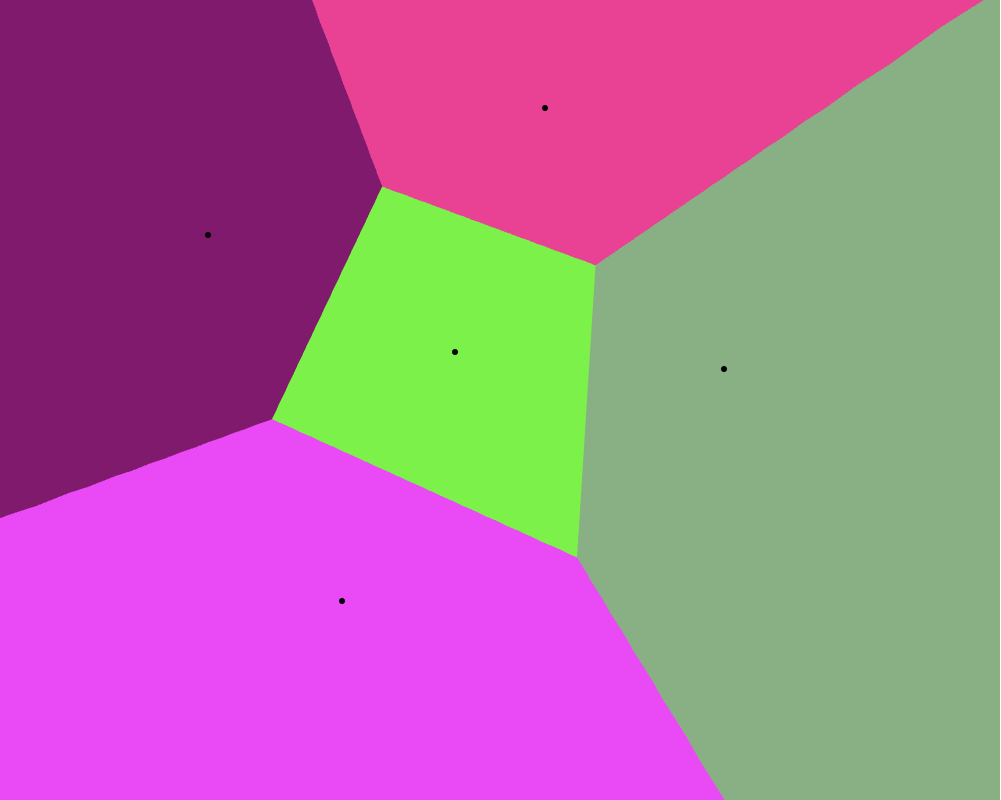
\includegraphics[scale = 0.4]{Диаграмма для задачи}
\end{center}
\newpage
\section{Формальная постановка задачи}
\begin{enumerate}
\item Изучить алгоритм Форчуна, описать его в форме научного доклада...
\item Реализовать версию алгоритма Форчуна с его визуализированным изображением.(*добавить подробности)
\item Исследовать алгоритм на предельно допустимое количество входных данных.
\item Результаты работы выложить на гитхаб
\end{enumerate}


%1)Изучить....(структуру данных, что-нибудь еще, а потом название) и Описать ее\его в форме научного доклада 
%2)Реализовать алгоритм такой-то четко точно(может быть с использованием чего-то(библиотеки, доп алгоса))(операции которые реализуем расписать), ограничения(память\скорость\визуализация) на входные данные, Визуализация(если есть) в такой-то форме
%3)Выполнить исследование(исслед на предмет (производительности наприм.). /Тут таблички, графики, короче статистика, ВЫВОД из этого всего- уже в самом анализе/
%4Результаты работы выложить на гитхаб


%*сделать презентацию
%**

\section{Реализация}

\section{Список литературы}
\begin{enumerate}
\item Steven Fortune. A sweepline algorithm for Voronoi diagrams // ACM Digital Library Proceedings of the second annual symposium on Computational geometry. — Yorktown Heights, New York, United States, 1986. — ISBN 0-89791-194-6. 
\item Mark de Berg, Marc van Kreveld, Mark Overmars, Otfried Schwarzkopf. Computational Geometry. — 2nd revised. — Springer-Verlag, 2000. — ISBN 3-540-65620-0.
\item David Austin. Voronoi Diagrams and a Day at the Beach. — American Mathematical Society.
\item Rene Descartes, Le Monde, ou Traité de la lumière, Translation and introduction by M.S. Mahoney, Abaris, 1979.
\item A. Okabe, B. Boots, K. Sugihara, S. Chiu, Spatial Tesselations, Concepts and Applications of Voronoi Diagrams, Wiley, 2000.
\item J. O'Rourke, Computational Geometry in C, Cambridge University Press, 2000.
\item Spatial: диаграмма Вороного (Java) [Электронный ресурс] — Режим доступа: http://obi2ru.blogspot.com/2012/12/spatial-voronoi-diagram-by-java.html
\item Kenny Wong, Hausi A. Müller, An Efficient Implementation of Fortune's Plane-Sweep Algorithm for Voronoi Diagrams, CiteSeerX   10.1.1.83.5571 .
\item Wikipedia: Алгоритм Форчуна 
\item Javascript Implementation of Steven J. Fortune's Algorythm to compute Voronoi diagrams [Электронный ресус] — Режим доступа: http://www.raymondhill.net/voronoi/rhill-voronoi.html
\item Алгоритм Форчуна, подробности реализации [Электронный ресус] — Режим доступа: https://habr.com/ru/post/430628/
\item Ход «Voronoi» [Электронный ресус] — Режим доступа: https://habr.com/ru/post/110790/
\item Ход «Voronoi». Часть 2 — Бинарное дерево  [Электронный ресус] — Режим доступа: https://habr.com/ru/post/112581/
\item С++ для начинающих. Бинарное дерево. Первое знакомство [Электронный ресус] — Режим доступа: https://ci-plus-plus-snachala.ru/?p=89
\item Практика метапрограммирования на C++: бинарное дерево поиска на этапе компиляции [Электронный ресус] — Режим доступа: https://habr.com/ru/p ost/320686/
\item Fortune's Algorithm in C++ [Электронный ресус] — Режим доступа: https://www.cs.hmc.edu/-mbrubeck/voronoi.html
\item Voronoi diagrams with Fortune's algorithm  [Электронный ресус] — Режим доступа: https://www.bitbanging.space/posts/voronoi-diagram-with-fortunes-algorithm
\item Wikipedia: Fortune's algorithm
\item Fortune's algorithm  [Электронный ресус] — Режим доступа: https://wikimili.com/en/Fortune's-algorithm
\item Диаграмма Вороного и её применения [Электронный ресус] — Режим доступа: https://itnan.ru/post.php?c=1&p=309252
\item Voronoi Diagrams and a Day at the Beach [Электронный ресус] — Режим доступа: https://www.ams.org/publicoutreach/feature-column/fcarc-voronoi
\item Voronoi diagram in AS3 [Электронный ресус] — Режим доступа: https://blog.ivank.net/voronoi-diagram-in-as3.html
\item Алгоритм Форчуна на C++ для построения диаграммы Вороного на плоскости [Электронный ресус] — Режим доступа: https://www.pvsm.ru/matematika/211589
\item THE BOOST.POLYGON VORONOI LIBRARY [Электронный ресус] — Режим доступа: https://www.boost.org/doc/libs/1-52-0/libs/polygon/doc/voronoi-main.htm
\item Voronoi Diagram using Fortune's Algorithm [Электронный ресус] — Режим доступа: https://www.youtube.com/watch?v=dgEt9Go7GvE
\item Voronoi Diagrams and Procedural Map Generation [Электронный ресус] — Режим доступа: https://www.youtube.com/watch?v=3G5d8ob-Lfo
\item Fortune's Algorithm: The Details [Электронный ресус] — Режим доступа: https://pvigier.github.io/2018/11/18/fortune-algorithm-details.html
\end{enumerate}

\end{document}
